\documentclass[twoside]{book}

% Packages required by doxygen
\usepackage{fixltx2e}
\usepackage{calc}
\usepackage{doxygen}
\usepackage[export]{adjustbox} % also loads graphicx
\usepackage{graphicx}
\usepackage[utf8]{inputenc}
\usepackage{makeidx}
\usepackage{multicol}
\usepackage{multirow}
\PassOptionsToPackage{warn}{textcomp}
\usepackage{textcomp}
\usepackage[nointegrals]{wasysym}
\usepackage[table]{xcolor}

% Font selection
\usepackage[T1]{fontenc}
\usepackage[scaled=.90]{helvet}
\usepackage{courier}
\usepackage{amssymb}
\usepackage{sectsty}
\renewcommand{\familydefault}{\sfdefault}
\allsectionsfont{%
  \fontseries{bc}\selectfont%
  \color{darkgray}%
}
\renewcommand{\DoxyLabelFont}{%
  \fontseries{bc}\selectfont%
  \color{darkgray}%
}
\newcommand{\+}{\discretionary{\mbox{\scriptsize$\hookleftarrow$}}{}{}}

% Page & text layout
\usepackage{geometry}
\geometry{%
  a4paper,%
  top=2.5cm,%
  bottom=2.5cm,%
  left=2.5cm,%
  right=2.5cm%
}
\tolerance=750
\hfuzz=15pt
\hbadness=750
\setlength{\emergencystretch}{15pt}
\setlength{\parindent}{0cm}
\setlength{\parskip}{3ex plus 2ex minus 2ex}
\makeatletter
\renewcommand{\paragraph}{%
  \@startsection{paragraph}{4}{0ex}{-1.0ex}{1.0ex}{%
    \normalfont\normalsize\bfseries\SS@parafont%
  }%
}
\renewcommand{\subparagraph}{%
  \@startsection{subparagraph}{5}{0ex}{-1.0ex}{1.0ex}{%
    \normalfont\normalsize\bfseries\SS@subparafont%
  }%
}
\makeatother

% Headers & footers
\usepackage{fancyhdr}
\pagestyle{fancyplain}
\fancyhead[LE]{\fancyplain{}{\bfseries\thepage}}
\fancyhead[CE]{\fancyplain{}{}}
\fancyhead[RE]{\fancyplain{}{\bfseries\leftmark}}
\fancyhead[LO]{\fancyplain{}{\bfseries\rightmark}}
\fancyhead[CO]{\fancyplain{}{}}
\fancyhead[RO]{\fancyplain{}{\bfseries\thepage}}
\fancyfoot[LE]{\fancyplain{}{}}
\fancyfoot[CE]{\fancyplain{}{}}
\fancyfoot[RE]{\fancyplain{}{\bfseries\scriptsize Generated by Doxygen }}
\fancyfoot[LO]{\fancyplain{}{\bfseries\scriptsize Generated by Doxygen }}
\fancyfoot[CO]{\fancyplain{}{}}
\fancyfoot[RO]{\fancyplain{}{}}
\renewcommand{\footrulewidth}{0.4pt}
\renewcommand{\chaptermark}[1]{%
  \markboth{#1}{}%
}
\renewcommand{\sectionmark}[1]{%
  \markright{\thesection\ #1}%
}

% Indices & bibliography
\usepackage{natbib}
\usepackage[titles]{tocloft}
\setcounter{tocdepth}{3}
\setcounter{secnumdepth}{5}
\makeindex

% Hyperlinks (required, but should be loaded last)
\usepackage{ifpdf}
\ifpdf
  \usepackage[pdftex,pagebackref=true]{hyperref}
\else
  \usepackage[ps2pdf,pagebackref=true]{hyperref}
\fi
\hypersetup{%
  colorlinks=true,%
  linkcolor=blue,%
  citecolor=blue,%
  unicode%
}

% Custom commands
\newcommand{\clearemptydoublepage}{%
  \newpage{\pagestyle{empty}\cleardoublepage}%
}

\usepackage{caption}
\captionsetup{labelsep=space,justification=centering,font={bf},singlelinecheck=off,skip=4pt,position=top}

%===== C O N T E N T S =====

\begin{document}

% Titlepage & ToC
\hypersetup{pageanchor=false,
             bookmarksnumbered=true,
             pdfencoding=unicode
            }
\pagenumbering{roman}
\begin{titlepage}
\vspace*{7cm}
\begin{center}%
{\Large F\+O\+S++ \\[1ex]\large 0.\+1 }\\
\vspace*{1cm}
{\large Generated by Doxygen 1.8.11}\\
\end{center}
\end{titlepage}
\clearemptydoublepage
\tableofcontents
\clearemptydoublepage
\pagenumbering{arabic}
\hypersetup{pageanchor=true}

%--- Begin generated contents ---
\chapter{Class Index}
\section{Class List}
Here are the classes, structs, unions and interfaces with brief descriptions\+:\begin{DoxyCompactList}
\item\contentsline{section}{\hyperlink{class_f_o_s}{F\+O\+S$<$ T $>$} \\*The main \hyperlink{class_f_o_s}{F\+OS} algorithim }{\pageref{class_f_o_s}}{}
\end{DoxyCompactList}

\chapter{File Index}
\section{File List}
Here is a list of all documented files with brief descriptions\+:\begin{DoxyCompactList}
\item\contentsline{section}{/home/bephillips2/\+Qt-\/\+Projects/\+F\+O\+S\+Redux/{\bfseries main.\+cpp} }{\pageref{main_8cpp}}{}
\item\contentsline{section}{/home/bephillips2/\+Qt-\/\+Projects/\+F\+O\+S\+Redux/{\bfseries test\+\_\+eigen3.\+h} }{\pageref{test__eigen3_8h}}{}
\item\contentsline{section}{/home/bephillips2/\+Qt-\/\+Projects/\+F\+O\+S\+Redux/\+F\+O\+S/{\bfseries fos.\+h} }{\pageref{fos_8h}}{}
\item\contentsline{section}{/home/bephillips2/\+Qt-\/\+Projects/\+F\+O\+S\+Redux/\+F\+O\+S/{\bfseries fos\+\_\+imperative.\+h} }{\pageref{fos__imperative_8h}}{}
\item\contentsline{section}{/home/bephillips2/\+Qt-\/\+Projects/\+F\+O\+S\+Redux/\+F\+O\+S/{\bfseries perf\+\_\+fos.\+h} }{\pageref{perf__fos_8h}}{}
\item\contentsline{section}{/home/bephillips2/\+Qt-\/\+Projects/\+F\+O\+S\+Redux/\+F\+O\+S/{\bfseries perf\+\_\+fos\+\_\+experimental.\+h} }{\pageref{perf__fos__experimental_8h}}{}
\item\contentsline{section}{/home/bephillips2/\+Qt-\/\+Projects/\+F\+O\+S\+Redux/\+F\+O\+S/{\bfseries test\+\_\+fos.\+h} }{\pageref{test__fos_8h}}{}
\item\contentsline{section}{/home/bephillips2/\+Qt-\/\+Projects/\+F\+O\+S\+Redux/\+F\+O\+S/{\bfseries test\+\_\+fos\+\_\+experimental.\+h} }{\pageref{test__fos__experimental_8h}}{}
\item\contentsline{section}{/home/bephillips2/\+Qt-\/\+Projects/\+F\+O\+S\+Redux/\+F\+O\+S/{\bfseries x\+\_\+fos.\+h} }{\pageref{x__fos_8h}}{}
\item\contentsline{section}{/home/bephillips2/\+Qt-\/\+Projects/\+F\+O\+S\+Redux/\+Generic/\hyperlink{algorithm_8h}{algorithm.\+h} \\*Functions that provide an interface between Eigen and Spams linear algebra libraries }{\pageref{algorithm_8h}}{}
\item\contentsline{section}{/home/bephillips2/\+Qt-\/\+Projects/\+F\+O\+S\+Redux/\+Generic/\hyperlink{debug_8h}{debug.\+h} \\*Preprocessor macros used for debugging and profiling }{\pageref{debug_8h}}{}
\item\contentsline{section}{/home/bephillips2/\+Qt-\/\+Projects/\+F\+O\+S\+Redux/\+Generic/\hyperlink{generics_8h}{generics.\+h} \\*Generic linear algebra functions }{\pageref{generics_8h}}{}
\item\contentsline{section}{/home/bephillips2/\+Qt-\/\+Projects/\+F\+O\+S\+Redux/\+I\+S\+T\+A/{\bfseries ista.\+h} }{\pageref{ista_8h}}{}
\item\contentsline{section}{/home/bephillips2/\+Qt-\/\+Projects/\+F\+O\+S\+Redux/\+I\+S\+T\+A/{\bfseries perf\+\_\+ista.\+h} }{\pageref{perf__ista_8h}}{}
\item\contentsline{section}{/home/bephillips2/\+Qt-\/\+Projects/\+F\+O\+S\+Redux/\+I\+S\+T\+A/{\bfseries test\+\_\+ista.\+h} }{\pageref{test__ista_8h}}{}
\item\contentsline{section}{/home/bephillips2/\+Qt-\/\+Projects/\+F\+O\+S\+Redux/\+Open\+C\+L\+\_\+\+Base/{\bfseries openclbase.\+cpp} }{\pageref{openclbase_8cpp}}{}
\item\contentsline{section}{/home/bephillips2/\+Qt-\/\+Projects/\+F\+O\+S\+Redux/\+Open\+C\+L\+\_\+\+Base/{\bfseries openclbase.\+h} }{\pageref{openclbase_8h}}{}
\item\contentsline{section}{/home/bephillips2/\+Qt-\/\+Projects/\+F\+O\+S\+Redux/\+Open\+C\+L\+\_\+\+Generics/{\bfseries cl\+\_\+algorithm.\+h} }{\pageref{cl__algorithm_8h}}{}
\item\contentsline{section}{/home/bephillips2/\+Qt-\/\+Projects/\+F\+O\+S\+Redux/\+Open\+C\+L\+\_\+\+Generics/{\bfseries cl\+\_\+generics.\+h} }{\pageref{cl__generics_8h}}{}
\item\contentsline{section}{/home/bephillips2/\+Qt-\/\+Projects/\+F\+O\+S\+Redux/\+Open\+C\+L\+\_\+\+Generics/{\bfseries perf\+\_\+cl\+\_\+product.\+cpp} }{\pageref{perf__cl__product_8cpp}}{}
\item\contentsline{section}{/home/bephillips2/\+Qt-\/\+Projects/\+F\+O\+S\+Redux/\+Open\+C\+L\+\_\+\+Generics/{\bfseries perf\+\_\+cl\+\_\+product.\+h} }{\pageref{perf__cl__product_8h}}{}
\item\contentsline{section}{/home/bephillips2/\+Qt-\/\+Projects/\+F\+O\+S\+Redux/\+S\+P\+A\+M\+S/{\bfseries perf\+\_\+fista.\+h} }{\pageref{perf__fista_8h}}{}
\item\contentsline{section}{/home/bephillips2/\+Qt-\/\+Projects/\+F\+O\+S\+Redux/\+S\+P\+A\+M\+S/{\bfseries test\+\_\+fista.\+h} }{\pageref{test__fista_8h}}{}
\end{DoxyCompactList}

\chapter{Class Documentation}
\hypertarget{class_f_o_s}{}\section{F\+OS$<$ T $>$ Class Template Reference}
\label{class_f_o_s}\index{F\+O\+S$<$ T $>$@{F\+O\+S$<$ T $>$}}


The main \hyperlink{class_f_o_s}{F\+OS} algorithim.  




{\ttfamily \#include $<$fos.\+h$>$}

\subsection*{Public Member Functions}
\begin{DoxyCompactItemize}
\item 
\hyperlink{class_f_o_s_afe9890a8ccc16999cb8175539ae6eedd}{F\+OS} (Eigen\+::\+Matrix$<$ T, Eigen\+::\+Dynamic, Eigen\+::\+Dynamic $>$ x, Eigen\+::\+Matrix$<$ T, Eigen\+::\+Dynamic, 1 $>$ y)
\begin{DoxyCompactList}\small\item\em Initialize a new algorithm, and instantiate member attributes X and Y. \end{DoxyCompactList}\item 
void \hyperlink{class_f_o_s_a18a5f85f95eb2cefe26fb25d13127c38}{Algorithm} ()
\begin{DoxyCompactList}\small\item\em Run the main \hyperlink{class_f_o_s}{F\+OS} algorithm. \end{DoxyCompactList}\end{DoxyCompactItemize}


\subsection{Detailed Description}
\subsubsection*{template$<$typename T$>$\\*
class F\+O\+S$<$ T $>$}

The main \hyperlink{class_f_o_s}{F\+OS} algorithim. 

Definition at line 23 of file fos.\+h.



\subsection{Constructor \& Destructor Documentation}
\index{F\+OS@{F\+OS}!F\+OS@{F\+OS}}
\index{F\+OS@{F\+OS}!F\+OS@{F\+OS}}
\subsubsection[{\texorpdfstring{F\+O\+S(\+Eigen\+::\+Matrix$<$ T, Eigen\+::\+Dynamic, Eigen\+::\+Dynamic $>$ x, Eigen\+::\+Matrix$<$ T, Eigen\+::\+Dynamic, 1 $>$ y)}{FOS(Eigen::Matrix< T, Eigen::Dynamic, Eigen::Dynamic > x, Eigen::Matrix< T, Eigen::Dynamic, 1 > y)}}]{\setlength{\rightskip}{0pt plus 5cm}template$<$typename T $>$ {\bf F\+OS}$<$ T $>$\+::{\bf F\+OS} (
\begin{DoxyParamCaption}
\item[{Eigen\+::\+Matrix$<$ T, Eigen\+::\+Dynamic, Eigen\+::\+Dynamic $>$}]{x, }
\item[{Eigen\+::\+Matrix$<$ T, Eigen\+::\+Dynamic, 1 $>$}]{y}
\end{DoxyParamCaption}
)}\hypertarget{class_f_o_s_afe9890a8ccc16999cb8175539ae6eedd}{}\label{class_f_o_s_afe9890a8ccc16999cb8175539ae6eedd}


Initialize a new algorithm, and instantiate member attributes X and Y. 


\begin{DoxyParams}{Parameters}
{\em x} & An n x p design matrix\\
\hline
{\em y} & An n x 1 vector \\
\hline
\end{DoxyParams}


Definition at line 63 of file fos.\+h.



\subsection{Member Function Documentation}
\index{F\+OS@{F\+OS}!Algorithm@{Algorithm}}
\index{Algorithm@{Algorithm}!F\+OS@{F\+OS}}
\subsubsection[{\texorpdfstring{Algorithm()}{Algorithm()}}]{\setlength{\rightskip}{0pt plus 5cm}template$<$typename T $>$ void {\bf F\+OS}$<$ T $>$\+::Algorithm (
\begin{DoxyParamCaption}
{}
\end{DoxyParamCaption}
)}\hypertarget{class_f_o_s_a18a5f85f95eb2cefe26fb25d13127c38}{}\label{class_f_o_s_a18a5f85f95eb2cefe26fb25d13127c38}


Run the main \hyperlink{class_f_o_s}{F\+OS} algorithm. 

Calling this function will run the \hyperlink{class_f_o_s}{F\+OS} algorithm using the values of X and Y that were instantiated with the class constructor. 

Definition at line 268 of file fos.\+h.


\chapter{File Documentation}
\hypertarget{fos__generics_8h}{}\section{/home/bephillips2/\+Qt-\/\+Projects/\+F\+O\+S\+Redux/fos\+\_\+generics.h File Reference}
\label{fos__generics_8h}\index{/home/bephillips2/\+Qt-\/\+Projects/\+F\+O\+S\+Redux/fos\+\_\+generics.\+h@{/home/bephillips2/\+Qt-\/\+Projects/\+F\+O\+S\+Redux/fos\+\_\+generics.\+h}}


Generic linear algebra functions.  


{\ttfamily \#include $<$eigen3/\+Eigen/\+Dense$>$}\\*
{\ttfamily \#include $<$armadillo$>$}\\*
Include dependency graph for fos\+\_\+generics.\+h\+:\nopagebreak
\begin{figure}[H]
\begin{center}
\leavevmode
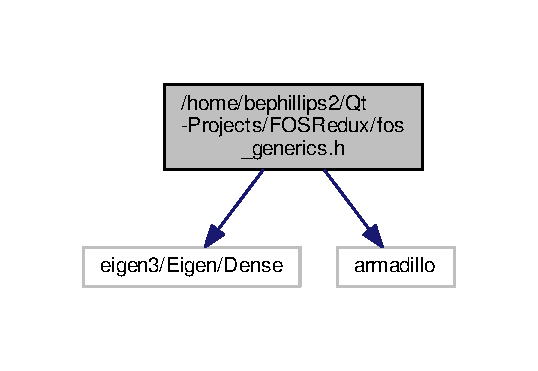
\includegraphics[width=258pt]{fos__generics_8h__incl}
\end{center}
\end{figure}
This graph shows which files directly or indirectly include this file\+:\nopagebreak
\begin{figure}[H]
\begin{center}
\leavevmode
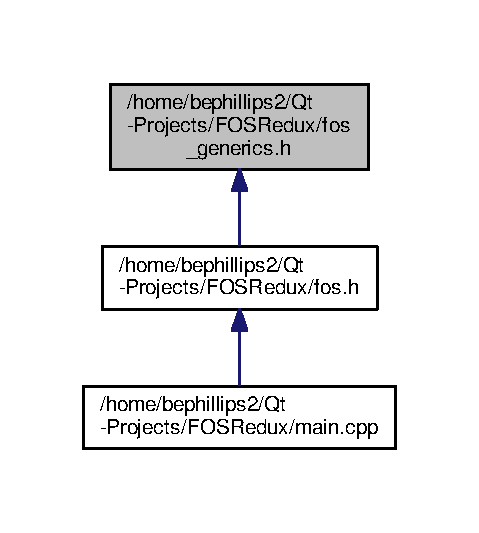
\includegraphics[width=230pt]{fos__generics_8h__dep__incl}
\end{center}
\end{figure}
\subsection*{Functions}
\begin{DoxyCompactItemize}
\item 
{\footnotesize template$<$typename T $>$ }\\T \hyperlink{fos__generics_8h_a3078b76bc228add250f305d3e877cf22}{C\+S\+V2\+Eigen} (std\+::string file\+\_\+path)
\begin{DoxyCompactList}\small\item\em Read a .csv file into an Eigen Matrix. \end{DoxyCompactList}\item 
void {\bfseries remove\+Row} (Eigen\+::\+Matrix\+Xd \&matrix, unsigned int row\+To\+Remove)\hypertarget{fos__generics_8h_a9a8df2e00594376f2c7ffb25988813d7}{}\label{fos__generics_8h_a9a8df2e00594376f2c7ffb25988813d7}

\item 
void {\bfseries remove\+Column} (Eigen\+::\+Matrix\+Xd \&matrix, unsigned int col\+To\+Remove)\hypertarget{fos__generics_8h_a05a555e2f83d10928a5a7202009f4f2f}{}\label{fos__generics_8h_a05a555e2f83d10928a5a7202009f4f2f}

\item 
{\footnotesize template$<$typename T $>$ }\\T \hyperlink{fos__generics_8h_ab660c06caa624c4213e9a8fc81f05bbb}{Std\+Dev} (const Eigen\+::\+Matrix$<$ T, Eigen\+::\+Dynamic, Eigen\+::\+Dynamic $>$ \&mat)
\begin{DoxyCompactList}\small\item\em Compute the standard deviation of a matrix. \end{DoxyCompactList}\item 
{\footnotesize template$<$typename T $>$ }\\void \hyperlink{fos__generics_8h_a344f938a854d73b7f8601510b9b56572}{Normalize} (Eigen\+::\+Matrix$<$ T, Eigen\+::\+Dynamic, Eigen\+::\+Dynamic $>$ \&mat)
\begin{DoxyCompactList}\small\item\em Set the mean of a matrix to 0 and the standard deviation to 1. \end{DoxyCompactList}\item 
{\footnotesize template$<$typename T $>$ }\\void \hyperlink{fos__generics_8h_a48e19f4572493cb8903c79b94a88e182}{Normalize} (Eigen\+::\+Matrix$<$ T, Eigen\+::\+Dynamic, 1 $>$ \&mat)
\begin{DoxyCompactList}\small\item\em Set the mean of a vector to 0 and the standard deviation to 1. \end{DoxyCompactList}\end{DoxyCompactItemize}


\subsection{Detailed Description}
Generic linear algebra functions. 



\subsection{Function Documentation}
\index{fos\+\_\+generics.\+h@{fos\+\_\+generics.\+h}!C\+S\+V2\+Eigen@{C\+S\+V2\+Eigen}}
\index{C\+S\+V2\+Eigen@{C\+S\+V2\+Eigen}!fos\+\_\+generics.\+h@{fos\+\_\+generics.\+h}}
\subsubsection[{\texorpdfstring{C\+S\+V2\+Eigen(std\+::string file\+\_\+path)}{CSV2Eigen(std::string file_path)}}]{\setlength{\rightskip}{0pt plus 5cm}template$<$typename T $>$ T C\+S\+V2\+Eigen (
\begin{DoxyParamCaption}
\item[{std\+::string}]{file\+\_\+path}
\end{DoxyParamCaption}
)}\hypertarget{fos__generics_8h_a3078b76bc228add250f305d3e877cf22}{}\label{fos__generics_8h_a3078b76bc228add250f305d3e877cf22}


Read a .csv file into an Eigen Matrix. 

Files must -\/not-\/ have header information of any kind (e.\+g. row/col labels etc. ) Rows are determined by line breakers, columns are determined by comma-\/delimiter.


\begin{DoxyParams}{Parameters}
{\em file\+\_\+path} & The (hard) path to the data file.\\
\hline
\end{DoxyParams}
\begin{DoxyReturn}{Returns}
An Eigen matrix with rows/cols determined by data file. 
\end{DoxyReturn}


Definition at line 37 of file fos\+\_\+generics.\+h.

\index{fos\+\_\+generics.\+h@{fos\+\_\+generics.\+h}!Normalize@{Normalize}}
\index{Normalize@{Normalize}!fos\+\_\+generics.\+h@{fos\+\_\+generics.\+h}}
\subsubsection[{\texorpdfstring{Normalize(\+Eigen\+::\+Matrix$<$ T, Eigen\+::\+Dynamic, Eigen\+::\+Dynamic $>$ \&mat)}{Normalize(Eigen::Matrix< T, Eigen::Dynamic, Eigen::Dynamic > &mat)}}]{\setlength{\rightskip}{0pt plus 5cm}template$<$typename T $>$ void Normalize (
\begin{DoxyParamCaption}
\item[{Eigen\+::\+Matrix$<$ T, Eigen\+::\+Dynamic, Eigen\+::\+Dynamic $>$ \&}]{mat}
\end{DoxyParamCaption}
)}\hypertarget{fos__generics_8h_a344f938a854d73b7f8601510b9b56572}{}\label{fos__generics_8h_a344f938a854d73b7f8601510b9b56572}


Set the mean of a matrix to 0 and the standard deviation to 1. 

Note this function is done in place, that is the input matrix is modified.


\begin{DoxyParams}{Parameters}
{\em mat} & An n x m matrix to be normalized. \\
\hline
\end{DoxyParams}


Definition at line 105 of file fos\+\_\+generics.\+h.

\index{fos\+\_\+generics.\+h@{fos\+\_\+generics.\+h}!Normalize@{Normalize}}
\index{Normalize@{Normalize}!fos\+\_\+generics.\+h@{fos\+\_\+generics.\+h}}
\subsubsection[{\texorpdfstring{Normalize(\+Eigen\+::\+Matrix$<$ T, Eigen\+::\+Dynamic, 1 $>$ \&mat)}{Normalize(Eigen::Matrix< T, Eigen::Dynamic, 1 > &mat)}}]{\setlength{\rightskip}{0pt plus 5cm}template$<$typename T $>$ void Normalize (
\begin{DoxyParamCaption}
\item[{Eigen\+::\+Matrix$<$ T, Eigen\+::\+Dynamic, 1 $>$ \&}]{mat}
\end{DoxyParamCaption}
)}\hypertarget{fos__generics_8h_a48e19f4572493cb8903c79b94a88e182}{}\label{fos__generics_8h_a48e19f4572493cb8903c79b94a88e182}


Set the mean of a vector to 0 and the standard deviation to 1. 

Note this function is done in place.


\begin{DoxyParams}{Parameters}
{\em mat} & An n x 1 vector to be normalized. \\
\hline
\end{DoxyParams}


Definition at line 123 of file fos\+\_\+generics.\+h.

\index{fos\+\_\+generics.\+h@{fos\+\_\+generics.\+h}!Std\+Dev@{Std\+Dev}}
\index{Std\+Dev@{Std\+Dev}!fos\+\_\+generics.\+h@{fos\+\_\+generics.\+h}}
\subsubsection[{\texorpdfstring{Std\+Dev(const Eigen\+::\+Matrix$<$ T, Eigen\+::\+Dynamic, Eigen\+::\+Dynamic $>$ \&mat)}{StdDev(const Eigen::Matrix< T, Eigen::Dynamic, Eigen::Dynamic > &mat)}}]{\setlength{\rightskip}{0pt plus 5cm}template$<$typename T $>$ T Std\+Dev (
\begin{DoxyParamCaption}
\item[{const Eigen\+::\+Matrix$<$ T, Eigen\+::\+Dynamic, Eigen\+::\+Dynamic $>$ \&}]{mat}
\end{DoxyParamCaption}
)}\hypertarget{fos__generics_8h_ab660c06caa624c4213e9a8fc81f05bbb}{}\label{fos__generics_8h_ab660c06caa624c4213e9a8fc81f05bbb}


Compute the standard deviation of a matrix. 


\begin{DoxyParams}{Parameters}
{\em mat} & Matrix to be examined.\\
\hline
\end{DoxyParams}
\begin{DoxyReturn}{Returns}
Standard deviation of the matrix 
\end{DoxyReturn}


Definition at line 88 of file fos\+\_\+generics.\+h.


\hypertarget{fos__typetraits_8h}{}\section{/home/bephillips2/\+Qt-\/\+Projects/\+F\+O\+S\+Redux/fos\+\_\+typetraits.h File Reference}
\label{fos__typetraits_8h}\index{/home/bephillips2/\+Qt-\/\+Projects/\+F\+O\+S\+Redux/fos\+\_\+typetraits.\+h@{/home/bephillips2/\+Qt-\/\+Projects/\+F\+O\+S\+Redux/fos\+\_\+typetraits.\+h}}


Preprocessor macros used for debugging and profiling.  


This graph shows which files directly or indirectly include this file\+:\nopagebreak
\begin{figure}[H]
\begin{center}
\leavevmode
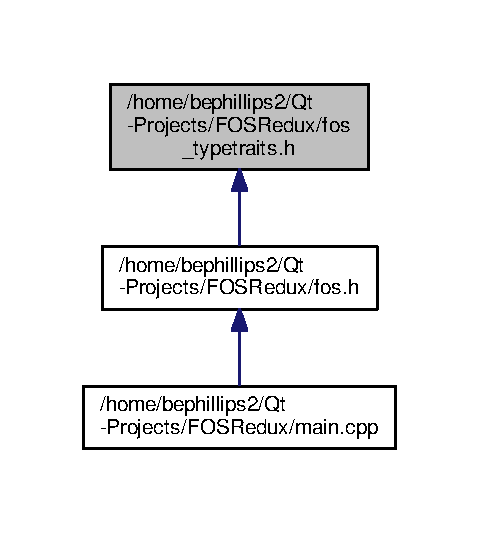
\includegraphics[width=230pt]{fos__typetraits_8h__dep__incl}
\end{center}
\end{figure}
\subsection*{Macros}
\begin{DoxyCompactItemize}
\item 
\#define \hyperlink{fos__typetraits_8h_ae7cd57cebd2ba2707f8d54ef09abbd12}{T\+I\+M\+E\+\_\+\+IT}(func, ...)
\item 
\#define \hyperlink{fos__typetraits_8h_af6551f0b4c3964c3128f808e7bf987c7}{D\+E\+B\+U\+G\+\_\+\+P\+R\+I\+NT}(x)~do \{\} while (0)
\end{DoxyCompactItemize}


\subsection{Detailed Description}
Preprocessor macros used for debugging and profiling. 



\subsection{Macro Definition Documentation}
\index{fos\+\_\+typetraits.\+h@{fos\+\_\+typetraits.\+h}!D\+E\+B\+U\+G\+\_\+\+P\+R\+I\+NT@{D\+E\+B\+U\+G\+\_\+\+P\+R\+I\+NT}}
\index{D\+E\+B\+U\+G\+\_\+\+P\+R\+I\+NT@{D\+E\+B\+U\+G\+\_\+\+P\+R\+I\+NT}!fos\+\_\+typetraits.\+h@{fos\+\_\+typetraits.\+h}}
\subsubsection[{\texorpdfstring{D\+E\+B\+U\+G\+\_\+\+P\+R\+I\+NT}{DEBUG_PRINT}}]{\setlength{\rightskip}{0pt plus 5cm}\#define D\+E\+B\+U\+G\+\_\+\+P\+R\+I\+NT(
\begin{DoxyParamCaption}
\item[{}]{x}
\end{DoxyParamCaption}
)~do \{\} while (0)}\hypertarget{fos__typetraits_8h_af6551f0b4c3964c3128f808e7bf987c7}{}\label{fos__typetraits_8h_af6551f0b4c3964c3128f808e7bf987c7}
Print a sequence of statements if program is compilied with the -\/\+D\+D\+E\+B\+UG flag. 

Definition at line 23 of file fos\+\_\+typetraits.\+h.

\index{fos\+\_\+typetraits.\+h@{fos\+\_\+typetraits.\+h}!T\+I\+M\+E\+\_\+\+IT@{T\+I\+M\+E\+\_\+\+IT}}
\index{T\+I\+M\+E\+\_\+\+IT@{T\+I\+M\+E\+\_\+\+IT}!fos\+\_\+typetraits.\+h@{fos\+\_\+typetraits.\+h}}
\subsubsection[{\texorpdfstring{T\+I\+M\+E\+\_\+\+IT}{TIME_IT}}]{\setlength{\rightskip}{0pt plus 5cm}\#define T\+I\+M\+E\+\_\+\+IT(
\begin{DoxyParamCaption}
\item[{}]{func, }
\item[{}]{...}
\end{DoxyParamCaption}
)}\hypertarget{fos__typetraits_8h_ae7cd57cebd2ba2707f8d54ef09abbd12}{}\label{fos__typetraits_8h_ae7cd57cebd2ba2707f8d54ef09abbd12}
{\bfseries Value\+:}
\begin{DoxyCode}
\textcolor{keywordflow}{do} \{ \(\backslash\)
        auto start = std::chrono::high\_resolution\_clock::now(); \(\backslash\)
        func \(\backslash\)
        auto end = std::chrono::high\_resolution\_clock::now();\(\backslash\)
        std::chrono::duration<double, std::milli> ms = end - start;\(\backslash\)
        auto time\_taken = ms.count();\(\backslash\)
        std::cout<< \textcolor{stringliteral}{"Function took "} << time\_taken <<\textcolor{stringliteral}{" ms."} << std::endl;\(\backslash\)
    \} \textcolor{keywordflow}{while} (0)
\end{DoxyCode}
Measure how long a function takes to execute. 

Definition at line 9 of file fos\+\_\+typetraits.\+h.


\hypertarget{fosalgorithm_8h}{}\section{/home/bephillips2/\+Qt-\/\+Projects/\+F\+O\+S\+Redux/fosalgorithm.h File Reference}
\label{fosalgorithm_8h}\index{/home/bephillips2/\+Qt-\/\+Projects/\+F\+O\+S\+Redux/fosalgorithm.\+h@{/home/bephillips2/\+Qt-\/\+Projects/\+F\+O\+S\+Redux/fosalgorithm.\+h}}


Functions that provide an interface between Eigen and Spams linear algebra libraries.  


{\ttfamily \#include $<$eigen3/\+Eigen/\+Dense$>$}\\*
{\ttfamily \#include \char`\"{}linalg.\+h\char`\"{}}\\*
{\ttfamily \#include \char`\"{}spams.\+h\char`\"{}}\\*
{\ttfamily \#include $<$armadillo$>$}\\*
Include dependency graph for fosalgorithm.\+h\+:\nopagebreak
\begin{figure}[H]
\begin{center}
\leavevmode
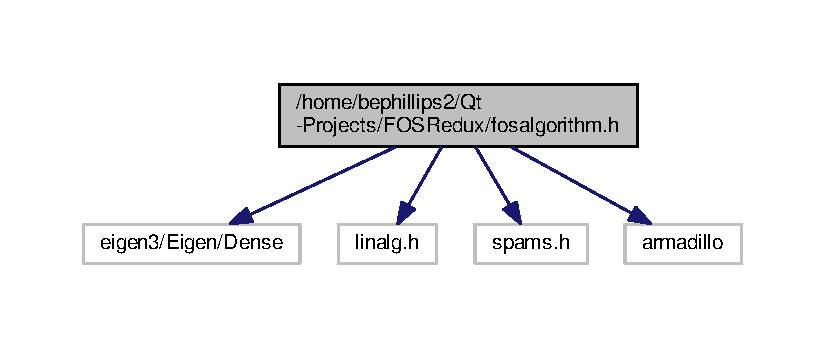
\includegraphics[width=350pt]{fosalgorithm_8h__incl}
\end{center}
\end{figure}
This graph shows which files directly or indirectly include this file\+:\nopagebreak
\begin{figure}[H]
\begin{center}
\leavevmode
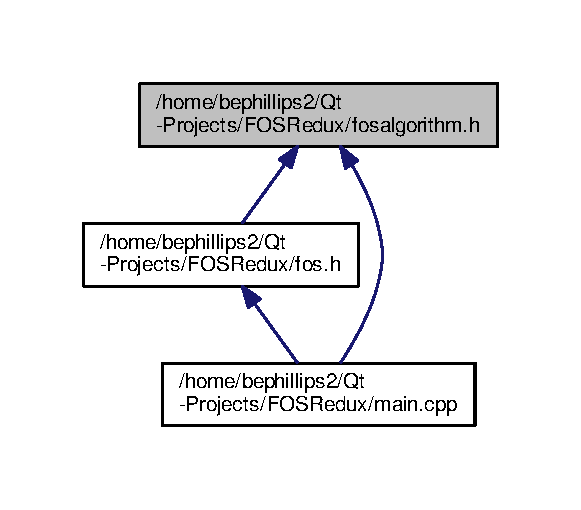
\includegraphics[width=279pt]{fosalgorithm_8h__dep__incl}
\end{center}
\end{figure}
\subsection*{Functions}
\begin{DoxyCompactItemize}
\item 
{\footnotesize template$<$typename T , uint m, uint n$>$ }\\Eigen\+::\+Matrix$<$ T, m, n $>$ \hyperlink{fosalgorithm_8h_a9b8b7c1219c57203eb55be82f363963d}{Spams2\+Eigen\+Mat} (const Matrix$<$ T $>$ $\ast$spams\+\_\+mat)
\begin{DoxyCompactList}\small\item\em Convert a const-\/ Spams Matrix to an Eigen\+::\+Matrix. \end{DoxyCompactList}\item 
{\footnotesize template$<$typename T , uint m, uint n$>$ }\\Eigen\+::\+Matrix$<$ T, m, n $>$ \hyperlink{fosalgorithm_8h_af95efdd1e0c89e28ecade0ccc5f87c4c}{Spams2\+Eigen\+Mat} (Matrix$<$ T $>$ $\ast$spams\+\_\+mat)
\begin{DoxyCompactList}\small\item\em Convert a Spams Matrix to an Eigen\+::\+Matrix whose rows and cols are known at compile time. \end{DoxyCompactList}\item 
{\footnotesize template$<$typename T $>$ }\\Eigen\+::\+Matrix$<$ T, Eigen\+::\+Dynamic, Eigen\+::\+Dynamic $>$ \hyperlink{fosalgorithm_8h_af2cddac6a7add7116fba0a5dd4b1b4d4}{Spams2\+Eigen\+Mat} (Matrix$<$ T $>$ $\ast$spams\+\_\+mat)
\begin{DoxyCompactList}\small\item\em Convert a Spams Matrix to an Eigen\+::\+Matrix whose rows and cols are assigned at run time. \end{DoxyCompactList}\item 
{\footnotesize template$<$typename T , uint m, uint n$>$ }\\Matrix$<$ T $>$ $\ast$ \hyperlink{fosalgorithm_8h_a0528c7867564847d122280b44b3f258e}{Eigen2\+Spams\+Mat} (const Eigen\+::\+Matrix$<$ T, n, m $>$ \&eigen\+\_\+mat)
\begin{DoxyCompactList}\small\item\em Get a spams Matrix from an Eigen\+::\+Matrix whose dimensions are know at compile time. \end{DoxyCompactList}\item 
{\footnotesize template$<$typename T $>$ }\\Matrix$<$ T $>$ $\ast$ \hyperlink{fosalgorithm_8h_a649fff8025ef5541fb3ca2c51c32fd9b}{Eigen2\+Spams\+Mat} (const Eigen\+::\+Matrix$<$ T, Eigen\+::\+Dynamic, Eigen\+::\+Dynamic $>$ \&eigen\+\_\+mat)
\begin{DoxyCompactList}\small\item\em Get a spams Matrix from an Eigen\+::\+Matrix whose dimensions are determined at run time. \end{DoxyCompactList}\item 
{\footnotesize template$<$typename T , uint m, uint n$>$ }\\Abstract\+MatrixB$<$ T $>$ {\bfseries Eigen2\+Spams\+Abstract\+MatB} (const Eigen\+::\+Matrix$<$ T, n, m $>$ \&eigen\+\_\+mat)\hypertarget{fosalgorithm_8h_ac00680a032bd45b1786197f2310d3286}{}\label{fosalgorithm_8h_ac00680a032bd45b1786197f2310d3286}

\item 
char $\ast$ \hyperlink{fosalgorithm_8h_ad7e3333e39a51029e238c41705f6884d}{str\+\_\+to\+\_\+c\+\_\+ptr} (std\+::string \&str)
\begin{DoxyCompactList}\small\item\em Translate a std\+::string into a pointer to a char array. \end{DoxyCompactList}\item 
{\footnotesize template$<$typename T $>$ }\\Matrix$<$ T $>$ $\ast$ \hyperlink{fosalgorithm_8h_aa227b689faec11b0585dcff2c4c4b9cc}{internal\+::\+Fista\+Flat} (Matrix$<$ T $>$ $\ast$Y, Matrix$<$ T $>$ $\ast$X, Matrix$<$ T $>$ $\ast$Omega\+\_\+0, const T lambda\+\_\+1)
\begin{DoxyCompactList}\small\item\em Performed \+\_\+fista\+Flat on Spams objects, returning parameters useful for the \hyperlink{class_f_o_s}{F\+OS} algorithim. \end{DoxyCompactList}\item 
{\footnotesize template$<$typename T $>$ }\\Eigen\+::\+Matrix$<$ T, Eigen\+::\+Dynamic, Eigen\+::\+Dynamic $>$ \hyperlink{fosalgorithm_8h_a21fff1ab4c69ac9ffcad454ec263d9e6}{Fista\+Flat} (Eigen\+::\+Matrix$<$ T, Eigen\+::\+Dynamic, Eigen\+::\+Dynamic $>$ Y, Eigen\+::\+Matrix$<$ T, Eigen\+::\+Dynamic, Eigen\+::\+Dynamic $>$ X, Eigen\+::\+Matrix$<$ T, Eigen\+::\+Dynamic, Eigen\+::\+Dynamic $>$ Omega\+\_\+0, const T lambda\+\_\+1)
\begin{DoxyCompactList}\small\item\em Performed fista\+Flat on Eigen objects, returning parameters useful for the \hyperlink{class_f_o_s}{F\+OS} algorithim. \end{DoxyCompactList}\end{DoxyCompactItemize}


\subsection{Detailed Description}
Functions that provide an interface between Eigen and Spams linear algebra libraries. 



\subsection{Function Documentation}
\index{fosalgorithm.\+h@{fosalgorithm.\+h}!Eigen2\+Spams\+Mat@{Eigen2\+Spams\+Mat}}
\index{Eigen2\+Spams\+Mat@{Eigen2\+Spams\+Mat}!fosalgorithm.\+h@{fosalgorithm.\+h}}
\subsubsection[{\texorpdfstring{Eigen2\+Spams\+Mat(const Eigen\+::\+Matrix$<$ T, n, m $>$ \&eigen\+\_\+mat)}{Eigen2SpamsMat(const Eigen::Matrix< T, n, m > &eigen_mat)}}]{\setlength{\rightskip}{0pt plus 5cm}template$<$typename T , uint m, uint n$>$ Matrix$<$T$>$$\ast$ Eigen2\+Spams\+Mat (
\begin{DoxyParamCaption}
\item[{const Eigen\+::\+Matrix$<$ T, n, m $>$ \&}]{eigen\+\_\+mat}
\end{DoxyParamCaption}
)}\hypertarget{fosalgorithm_8h_a0528c7867564847d122280b44b3f258e}{}\label{fosalgorithm_8h_a0528c7867564847d122280b44b3f258e}


Get a spams Matrix from an Eigen\+::\+Matrix whose dimensions are know at compile time. 


\begin{DoxyParams}{Parameters}
{\em eigen\+\_\+mat} & The Eigen\+::\+Matrix to be copied.\\
\hline
\end{DoxyParams}
\begin{DoxyReturn}{Returns}
A new Spams Matrix ( in pointer form ). 
\end{DoxyReturn}


Definition at line 86 of file fosalgorithm.\+h.

\index{fosalgorithm.\+h@{fosalgorithm.\+h}!Eigen2\+Spams\+Mat@{Eigen2\+Spams\+Mat}}
\index{Eigen2\+Spams\+Mat@{Eigen2\+Spams\+Mat}!fosalgorithm.\+h@{fosalgorithm.\+h}}
\subsubsection[{\texorpdfstring{Eigen2\+Spams\+Mat(const Eigen\+::\+Matrix$<$ T, Eigen\+::\+Dynamic, Eigen\+::\+Dynamic $>$ \&eigen\+\_\+mat)}{Eigen2SpamsMat(const Eigen::Matrix< T, Eigen::Dynamic, Eigen::Dynamic > &eigen_mat)}}]{\setlength{\rightskip}{0pt plus 5cm}template$<$typename T $>$ Matrix$<$T$>$$\ast$ Eigen2\+Spams\+Mat (
\begin{DoxyParamCaption}
\item[{const Eigen\+::\+Matrix$<$ T, Eigen\+::\+Dynamic, Eigen\+::\+Dynamic $>$ \&}]{eigen\+\_\+mat}
\end{DoxyParamCaption}
)}\hypertarget{fosalgorithm_8h_a649fff8025ef5541fb3ca2c51c32fd9b}{}\label{fosalgorithm_8h_a649fff8025ef5541fb3ca2c51c32fd9b}


Get a spams Matrix from an Eigen\+::\+Matrix whose dimensions are determined at run time. 


\begin{DoxyParams}{Parameters}
{\em eigen\+\_\+mat} & The Eigen\+::\+Matrix to be copied.\\
\hline
\end{DoxyParams}
\begin{DoxyReturn}{Returns}
A new Spams Matrix ( in pointer form ). 
\end{DoxyReturn}


Definition at line 113 of file fosalgorithm.\+h.

\index{fosalgorithm.\+h@{fosalgorithm.\+h}!Fista\+Flat@{Fista\+Flat}}
\index{Fista\+Flat@{Fista\+Flat}!fosalgorithm.\+h@{fosalgorithm.\+h}}
\subsubsection[{\texorpdfstring{Fista\+Flat(\+Matrix$<$ T $>$ $\ast$\+Y, Matrix$<$ T $>$ $\ast$\+X, Matrix$<$ T $>$ $\ast$\+Omega\+\_\+0, const T lambda\+\_\+1)}{FistaFlat(Matrix< T > *Y, Matrix< T > *X, Matrix< T > *Omega_0, const T lambda_1)}}]{\setlength{\rightskip}{0pt plus 5cm}template$<$typename T $>$ Matrix$<$T$>$$\ast$ internal\+::\+Fista\+Flat (
\begin{DoxyParamCaption}
\item[{Matrix$<$ T $>$ $\ast$}]{Y, }
\item[{Matrix$<$ T $>$ $\ast$}]{X, }
\item[{Matrix$<$ T $>$ $\ast$}]{Omega\+\_\+0, }
\item[{const T}]{lambda\+\_\+1}
\end{DoxyParamCaption}
)}\hypertarget{fosalgorithm_8h_file_aa227b689faec11b0585dcff2c4c4b9cc}{}\label{fosalgorithm_8h_file_aa227b689faec11b0585dcff2c4c4b9cc}


Performed \+\_\+fista\+Flat on Spams objects, returning parameters useful for the \hyperlink{class_f_o_s}{F\+OS} algorithim. 


\begin{DoxyParams}{Parameters}
{\em Y} & A n x 1 vector \\
\hline
{\em X} & An n x m desgin matrix\\
\hline
{\em Omega\+\_\+0} & An n x 1 vector of initial guesses ( probably )\\
\hline
{\em lambda\+\_\+1} & Regularization parameter\\
\hline
\end{DoxyParams}
\begin{DoxyReturn}{Returns}
Omega, a 1 x n matrix 
\end{DoxyReturn}


Definition at line 181 of file fosalgorithm.\+h.

\index{fosalgorithm.\+h@{fosalgorithm.\+h}!Fista\+Flat@{Fista\+Flat}}
\index{Fista\+Flat@{Fista\+Flat}!fosalgorithm.\+h@{fosalgorithm.\+h}}
\subsubsection[{\texorpdfstring{Fista\+Flat(\+Eigen\+::\+Matrix$<$ T, Eigen\+::\+Dynamic, Eigen\+::\+Dynamic $>$ Y, Eigen\+::\+Matrix$<$ T, Eigen\+::\+Dynamic, Eigen\+::\+Dynamic $>$ X, Eigen\+::\+Matrix$<$ T, Eigen\+::\+Dynamic, Eigen\+::\+Dynamic $>$ Omega\+\_\+0, const T lambda\+\_\+1)}{FistaFlat(Eigen::Matrix< T, Eigen::Dynamic, Eigen::Dynamic > Y, Eigen::Matrix< T, Eigen::Dynamic, Eigen::Dynamic > X, Eigen::Matrix< T, Eigen::Dynamic, Eigen::Dynamic > Omega_0, const T lambda_1)}}]{\setlength{\rightskip}{0pt plus 5cm}template$<$typename T $>$ Eigen\+::\+Matrix$<$ T, Eigen\+::\+Dynamic, Eigen\+::\+Dynamic$>$ Fista\+Flat (
\begin{DoxyParamCaption}
\item[{Eigen\+::\+Matrix$<$ T, Eigen\+::\+Dynamic, Eigen\+::\+Dynamic $>$}]{Y, }
\item[{Eigen\+::\+Matrix$<$ T, Eigen\+::\+Dynamic, Eigen\+::\+Dynamic $>$}]{X, }
\item[{Eigen\+::\+Matrix$<$ T, Eigen\+::\+Dynamic, Eigen\+::\+Dynamic $>$}]{Omega\+\_\+0, }
\item[{const T}]{lambda\+\_\+1}
\end{DoxyParamCaption}
)}\hypertarget{fosalgorithm_8h_a21fff1ab4c69ac9ffcad454ec263d9e6}{}\label{fosalgorithm_8h_a21fff1ab4c69ac9ffcad454ec263d9e6}


Performed fista\+Flat on Eigen objects, returning parameters useful for the \hyperlink{class_f_o_s}{F\+OS} algorithim. 


\begin{DoxyParams}{Parameters}
{\em Y} & A n x 1 vector \\
\hline
{\em X} & An n x m desgin matrix\\
\hline
{\em Omega\+\_\+0} & An n x 1 vector of initial guesses\\
\hline
{\em lambda\+\_\+1} & Regularization parameter\\
\hline
\end{DoxyParams}
\begin{DoxyReturn}{Returns}
Omega, a 1 x n matrix 
\end{DoxyReturn}


Definition at line 280 of file fosalgorithm.\+h.

\index{fosalgorithm.\+h@{fosalgorithm.\+h}!Spams2\+Eigen\+Mat@{Spams2\+Eigen\+Mat}}
\index{Spams2\+Eigen\+Mat@{Spams2\+Eigen\+Mat}!fosalgorithm.\+h@{fosalgorithm.\+h}}
\subsubsection[{\texorpdfstring{Spams2\+Eigen\+Mat(const Matrix$<$ T $>$ $\ast$spams\+\_\+mat)}{Spams2EigenMat(const Matrix< T > *spams_mat)}}]{\setlength{\rightskip}{0pt plus 5cm}template$<$typename T , uint m, uint n$>$ Eigen\+::\+Matrix$<$ T, m, n $>$ Spams2\+Eigen\+Mat (
\begin{DoxyParamCaption}
\item[{const Matrix$<$ T $>$ $\ast$}]{spams\+\_\+mat}
\end{DoxyParamCaption}
)}\hypertarget{fosalgorithm_8h_a9b8b7c1219c57203eb55be82f363963d}{}\label{fosalgorithm_8h_a9b8b7c1219c57203eb55be82f363963d}


Convert a const-\/ Spams Matrix to an Eigen\+::\+Matrix. 


\begin{DoxyParams}{Parameters}
{\em spams\+\_\+mat} & Spams Matrix pointer to be translated.\\
\hline
\end{DoxyParams}
\begin{DoxyReturn}{Returns}
A new Eigen\+::\+Matrix with dimensions determined by the Spams Matrix. 
\end{DoxyReturn}


Definition at line 35 of file fosalgorithm.\+h.

\index{fosalgorithm.\+h@{fosalgorithm.\+h}!Spams2\+Eigen\+Mat@{Spams2\+Eigen\+Mat}}
\index{Spams2\+Eigen\+Mat@{Spams2\+Eigen\+Mat}!fosalgorithm.\+h@{fosalgorithm.\+h}}
\subsubsection[{\texorpdfstring{Spams2\+Eigen\+Mat(\+Matrix$<$ T $>$ $\ast$spams\+\_\+mat)}{Spams2EigenMat(Matrix< T > *spams_mat)}}]{\setlength{\rightskip}{0pt plus 5cm}template$<$typename T , uint m, uint n$>$ Eigen\+::\+Matrix$<$ T, m, n $>$ Spams2\+Eigen\+Mat (
\begin{DoxyParamCaption}
\item[{Matrix$<$ T $>$ $\ast$}]{spams\+\_\+mat}
\end{DoxyParamCaption}
)}\hypertarget{fosalgorithm_8h_af95efdd1e0c89e28ecade0ccc5f87c4c}{}\label{fosalgorithm_8h_af95efdd1e0c89e28ecade0ccc5f87c4c}


Convert a Spams Matrix to an Eigen\+::\+Matrix whose rows and cols are known at compile time. 


\begin{DoxyParams}{Parameters}
{\em spams\+\_\+mat} & Spams Matrix pointer to be translated.\\
\hline
\end{DoxyParams}
\begin{DoxyReturn}{Returns}
A new Eigen\+::\+Matrix with dimensions determined by the Spams Matrix. 
\end{DoxyReturn}


Definition at line 50 of file fosalgorithm.\+h.

\index{fosalgorithm.\+h@{fosalgorithm.\+h}!Spams2\+Eigen\+Mat@{Spams2\+Eigen\+Mat}}
\index{Spams2\+Eigen\+Mat@{Spams2\+Eigen\+Mat}!fosalgorithm.\+h@{fosalgorithm.\+h}}
\subsubsection[{\texorpdfstring{Spams2\+Eigen\+Mat(\+Matrix$<$ T $>$ $\ast$spams\+\_\+mat)}{Spams2EigenMat(Matrix< T > *spams_mat)}}]{\setlength{\rightskip}{0pt plus 5cm}template$<$typename T $>$ Eigen\+::\+Matrix$<$ T, Eigen\+::\+Dynamic, Eigen\+::\+Dynamic $>$ Spams2\+Eigen\+Mat (
\begin{DoxyParamCaption}
\item[{Matrix$<$ T $>$ $\ast$}]{spams\+\_\+mat}
\end{DoxyParamCaption}
)}\hypertarget{fosalgorithm_8h_af2cddac6a7add7116fba0a5dd4b1b4d4}{}\label{fosalgorithm_8h_af2cddac6a7add7116fba0a5dd4b1b4d4}


Convert a Spams Matrix to an Eigen\+::\+Matrix whose rows and cols are assigned at run time. 


\begin{DoxyParams}{Parameters}
{\em spams\+\_\+mat} & Spams Matrix pointer to be translated.\\
\hline
\end{DoxyParams}
\begin{DoxyReturn}{Returns}
A new Eigen\+::\+Matrix with dimensions determined by the Spams Matrix. 
\end{DoxyReturn}


Definition at line 67 of file fosalgorithm.\+h.

\index{fosalgorithm.\+h@{fosalgorithm.\+h}!str\+\_\+to\+\_\+c\+\_\+ptr@{str\+\_\+to\+\_\+c\+\_\+ptr}}
\index{str\+\_\+to\+\_\+c\+\_\+ptr@{str\+\_\+to\+\_\+c\+\_\+ptr}!fosalgorithm.\+h@{fosalgorithm.\+h}}
\subsubsection[{\texorpdfstring{str\+\_\+to\+\_\+c\+\_\+ptr(std\+::string \&str)}{str_to_c_ptr(std::string &str)}}]{\setlength{\rightskip}{0pt plus 5cm}char$\ast$ str\+\_\+to\+\_\+c\+\_\+ptr (
\begin{DoxyParamCaption}
\item[{std\+::string \&}]{str}
\end{DoxyParamCaption}
)}\hypertarget{fosalgorithm_8h_ad7e3333e39a51029e238c41705f6884d}{}\label{fosalgorithm_8h_ad7e3333e39a51029e238c41705f6884d}


Translate a std\+::string into a pointer to a char array. 

Used with Spams \textquotesingle{}print\textquotesingle{} functions.


\begin{DoxyParams}{Parameters}
{\em str} & String to be transformed\\
\hline
\end{DoxyParams}
\begin{DoxyReturn}{Returns}
char$\ast$ populated with data in str and null terminator, Note that the char$\ast$ will need to be deleted later 
\end{DoxyReturn}


Definition at line 149 of file fosalgorithm.\+h.


%--- End generated contents ---

% Index
\backmatter
\newpage
\phantomsection
\clearemptydoublepage
\addcontentsline{toc}{chapter}{Index}
\printindex

\end{document}
